%% ==============================================
%%                   Evaluation
%% ==============================================
%% Author: Fabian Sorn
%% ==============================================

\chapter{Evaluation}
\label{ch:evaluation}

In this chapter we will evaluate the framework we designed and developed in the
last two chapters. We will start by evaluating, if the implementation fits our
requirements, by implementing the use cases presented in chapter
\ref{ch:usecases} and investigating their results. This will be followed by an
evaluation of the performance overhead the framework is producing, by comparing
the results with a minimal PyQt application recreating the same use case.

%% ==============================================
%%          Use Case Implementation
%% ==============================================

\section{Use Case Implementation}

This section will focus on the implementation of the use cases described in
chapter \ref{ch:usecases} based on widgetmark and its plotting library
abstraction layer. To have an overview of the development of the performance
of each use case depending the increasing plot counts, curve counts or dataset
sizes, we will run each use case with different parameters. We will start with
smaller sizes and increase them until we reach the use cases demanded
requirements. As a minimum refresh rate we will take the update frequency of the
use case. We will set the goal frame rate to 60Hz, which matches most modern
monitors. As data we will take random points each redraw, so we can be sure that
we will get a full redraw every time. As a repeat count we will take a
reasonable big number of 2000 redraws. Additionally we will define a timeout
that can stop use cases which take an unexpected long amount of time. Each use
case will be tested against both PyQtGraph and Matplotlib.

All of our three use cases have a very common setup. To avoid duplicated code,
we will define a setup helper class next to the use cases, which each one can
take advantage of. The implementation of its widget setup function can be seen
in listing \ref{listing:application:usecases:helper}. This helper function is
responsible for initializing a given number of plots, curves and random data
sets.

\lstinputlisting[ 
    caption=Setup helper function for creating plots, visualization items and
    data sets,
    language=python,
    label=listing:application:usecases:helper,
    linerange={20-27, 43-57}
]{resources/widgetmark/benchCern.py}

\subsection{Distributed Oscilloscope for BE-CO-HT}

The Distributed Oscilloscope features a central plot containing up to 8 curves
displaying up to 100,000 points at a time. To handle the update frequency of 25
Hertz, we will need a minimum frame rate of 25 frames per second. Listing
\ref{listing:application:usecases:ht:params} shows the implementation of these
parameters in a use case class as class attributes.

\lstinputlisting[ 
    caption=Definition of the parameters for the BE-CO-HT use case.,
    language=python,
    label=listing:application:usecases:ht:params,
    linerange={73-74, 79-89}
]{resources/widgetmark/benchCern.py}

Listing \ref{listing:application:usecases:ht:methods} shows the implementation
of the widget setup and the operation. For the setup we use the helper function
defined in listing \ref{listing:application:usecases:helper}. Since we only
create a single plot, we return it as the widget to use. The next function is
our operation definition, where we choose data and display in in our created
plots. To choose data from our random data sets, we take the current redraw run
as an index, which can be accessed through the runtime context object, that
every use case has access to.

\lstinputlisting[ 
    caption=Widget setup and operation definition for the BE-CO-HT use case.,
    language=python,
    label=listing:application:usecases:ht:methods,
    linerange={91-106}
]{resources/widgetmark/benchCern.py}

\subsection{Monitoring Application for BE-OP-LHC}

Our second use case features one central plot containing up to 3000 curves
displaying up to 2 * 3600 points, which should be updated every second. Listing
\ref{listing:application:usecases:ht:params} shows the implementation of these
requirements as parameters in the use case class. Widget Setup and operation
definition do not differ from listing
\ref{listing:application:usecases:ht:methods}.

\lstinputlisting[ 
    caption=Definition of the parameters for the BE-OP-LHC use case.,
    language=python,
    label=listing:application:usecases:ht:params,
    linerange={109-110, 115-125}
]{resources/widgetmark/benchCern.py}

\subsection{Linac4 Source GUI for BE-CO-APS}

Compared to the prior two use cases, this use case features multiple plots,
which means we can extend our parameter list with another entry for the plot
count. The implementation of the parameters in the use case class is displayed
in \ref{listing:application:usecases:aps:params}.

\lstinputlisting[ 
    caption=Definition of the parameters for the BE-CO-APS use case.,
    language=python,
    label=listing:application:usecases:aps:params,
    linerange={145-146, 151-162}
]{resources/widgetmark/benchCern.py}

Using multiple Plots means as well, that we have to change our setup function
slightly as seen in \ref{listing:application:usecases:aps:methods} by wrapping
the plots in another \inlinecode{Python}{QtWidgets.QWidget} object, which has a
\inlinecode{Python}{QtWidgets.QGridLayout} set as its internal layout. This way
we can pass our plots bundled as one single widget to the benchmark window.

\lstinputlisting[ 
    caption=Widget setup and operation definition for the BE-CO-APS use case.,
    language=python,
    label=listing:application:usecases:aps:methods,
    linerange={164-181}
]{resources/widgetmark/benchCern.py}

\subsection{Results}

After our benchmarks are defined, we can execute them using the widgetmark
command line interface. To receive results closest to the conditions in the
later production environment, we will run the benchmarks on machines with
similar hardware configurations.

\begin{description}

    \item[CPU:] Intel Core i7 6700 with 4 Cores (8 Threads),
                3.4GHz Base Clockspeed,
                4.0GHz Maximum Clockspeed

    \item[RAM:] 32GB

    \item[GPU:] Intel HD 530 Integrated Graphics

    \item[OS:] 64bit CentOS7

\end{description}

The size of the testing window was 800 x 600 pixels on all executed use cases.
The tables \ref{tab:application:usecases:results:ht},
\ref{tab:application:usecases:results:lhc} and
\ref{tab:application:usecases:results:aps} show the recorded results on this
machine. As we can see, PyQtGraph does perform substantially better compared to
Matplotlib, but the use cases clearly reveal that both have their limits.
Especially on the load provided by the \gls{lhcop} use case, both are struggling
severely with frame rates as low as 0.0 FPS, which means that a single redraw of
the entire dataset was taking more than 20 seconds on average. An interaction
with the plot is impossible at this point. For both libraries the amount of
points or datasets should be heavily reduced in these scenarios to keep the user
interface interactive. From the two given libraries, PyQtGraph is still the
better choice when it comes representing large data sets, if interactive
rendering speeds are required.

%% ~~~~~~~~~~~~~~~~~ BE-CO-HT Use case ~~~~~~~~~~~~~~~~~~~~

\begin{table}[h]
\begin{center}

\captionof{table}{Results of the BE-CO-HT use case}
\label{tab:application:usecases:results:ht}

\begin{tabular}{llrrlrr}

\hline
Use Case  & Library    & Plots & Items & Type    & Dataset & Frame Rate  \\
\hline
BE-CO-HT  & PyQtGraph  & 1     & 1     & Curve   & 1000    & 861.6       \\
BE-CO-HT  & Matplotlib & 1     & 1     & Curve   & 1000    & 31.0        \\
BE-CO-HT  & PyQtGraph  & 1     & 1     & Curve   & 10000   & 150.7       \\
BE-CO-HT  & Matplotlib & 1     & 1     & Curve   & 10000   & 5.2         \\
BE-CO-HT  & PyQtGraph  & 1     & 1     & Curve   & 100000  & 24.7        \\
BE-CO-HT  & Matplotlib & 1     & 1     & Curve   & 100000  & 1.6         \\
\hline
BE-CO-HT  & PyQtGraph  & 1     & 4     & Curve   & 1000    & 434.9       \\
BE-CO-HT  & Matplotlib & 1     & 4     & Curve   & 1000    & 7.7         \\
BE-CO-HT  & PyQtGraph  & 1     & 4     & Curve   & 10000   & 95.6        \\
BE-CO-HT  & Matplotlib & 1     & 4     & Curve   & 10000   & 1.6         \\
BE-CO-HT  & PyQtGraph  & 1     & 4     & Curve   & 100000  & 9.3         \\
BE-CO-HT  & Matplotlib & 1     & 4     & Curve   & 100000  & 0.5         \\
\hline
BE-CO-HT  & PyQtGraph  & 1     & 8     & Curve   & 1000    & 256.5       \\
BE-CO-HT  & Matplotlib & 1     & 8     & Curve   & 1000    & 3.6         \\
BE-CO-HT  & PyQtGraph  & 1     & 8     & Curve   & 10000   & 59.2        \\
BE-CO-HT  & Matplotlib & 1     & 8     & Curve   & 10000   & 0.8         \\
BE-CO-HT  & PyQtGraph  & 1     & 8     & Curve   & 100000  & 5.8         \\
BE-CO-HT  & Matplotlib & 1     & 8     & Curve   & 100000  & 0.2         \\
\hline

\end{tabular}
\end{center}
\end{table}

%% ~~~~~~~~~~~~~~~~~ BE-OP-LHC Use case ~~~~~~~~~~~~~~~~~~~~

\begin{table}[h]
\begin{center}

\captionof{table}{Results of the BE-OP-LHC use case}
\label{tab:application:usecases:results:lhc}

\begin{tabular}{llrrlrr}

\hline
Use Case  & Library    & Plots & Items & Type    & Dataset & Frame Rate  \\
\hline
BE-OP-LHC & PyQtGraph  & 1     & 300   & Curve   & 720     & 10.5        \\
BE-OP-LHC & Matplotlib & 1     & 300   & Curve   & 720     & 0.0         \\
BE-OP-LHC & PyQtGraph  & 1     & 3000  & Curve   & 720     & 2.6         \\
BE-OP-LHC & Matplotlib & 1     & 3000  & Curve   & 720     & 0.0         \\
BE-OP-LHC & PyQtGraph  & 1     & 3000  & Curve   & 7200    & 0.9         \\
BE-OP-LHC & Matplotlib & 1     & 3000  & Curve   & 7200    & 0.0         \\
\hline

\end{tabular}
\end{center}
\end{table}

%% ~~~~~~~~~~~~~~~~~ BE-OP-APS Use case ~~~~~~~~~~~~~~~~~~~~

\begin{table}[h]
\begin{center}

\captionof{table}{Results of the BE-CO-APS use case}
\label{tab:application:usecases:results:aps}

\begin{tabular}{llrrlrr}

\hline
Use Case  & Library    & Plots & Items & Type    & Dataset & Frame Rate  \\
\hline
BE-CO-APS & PyQtGraph  & 1     & 3     & Scatter & 3000    & 15.9        \\
BE-CO-APS & Matplotlib & 1     & 3     & Scatter & 3000    & 9.6         \\
BE-CO-APS & PyQtGraph  & 4     & 3     & Scatter & 3000    & 3.9         \\
BE-CO-APS & Matplotlib & 4     & 3     & Scatter & 3000    & 2.4         \\
\hline

\end{tabular}
\end{center}
\end{table}

With the profiler activated we can investigate where most of the computing time
is spent. In the following we will for example have a look at the profiles
created for the use cases run with PyQtGraph with high amounts of data. For
plots containing curves with a high amount of data, this is mainly the paint
event handler of the graphics view, which handles repainting the plot every time
the plot gets changed or moved. In more detail, the translation of the raw data
to a \inlinecode{Python}{QtGui.QPainterPath} as well as the actual painting done
by Qt's GraphicsView Framework. Screenshot
\ref{fig:application:lhc:usecase:profile:ht} shows the profile of the \gls{ht}
use case presented by Snakeviz in the Browser.

\begin{figure}[h]
    \centering
    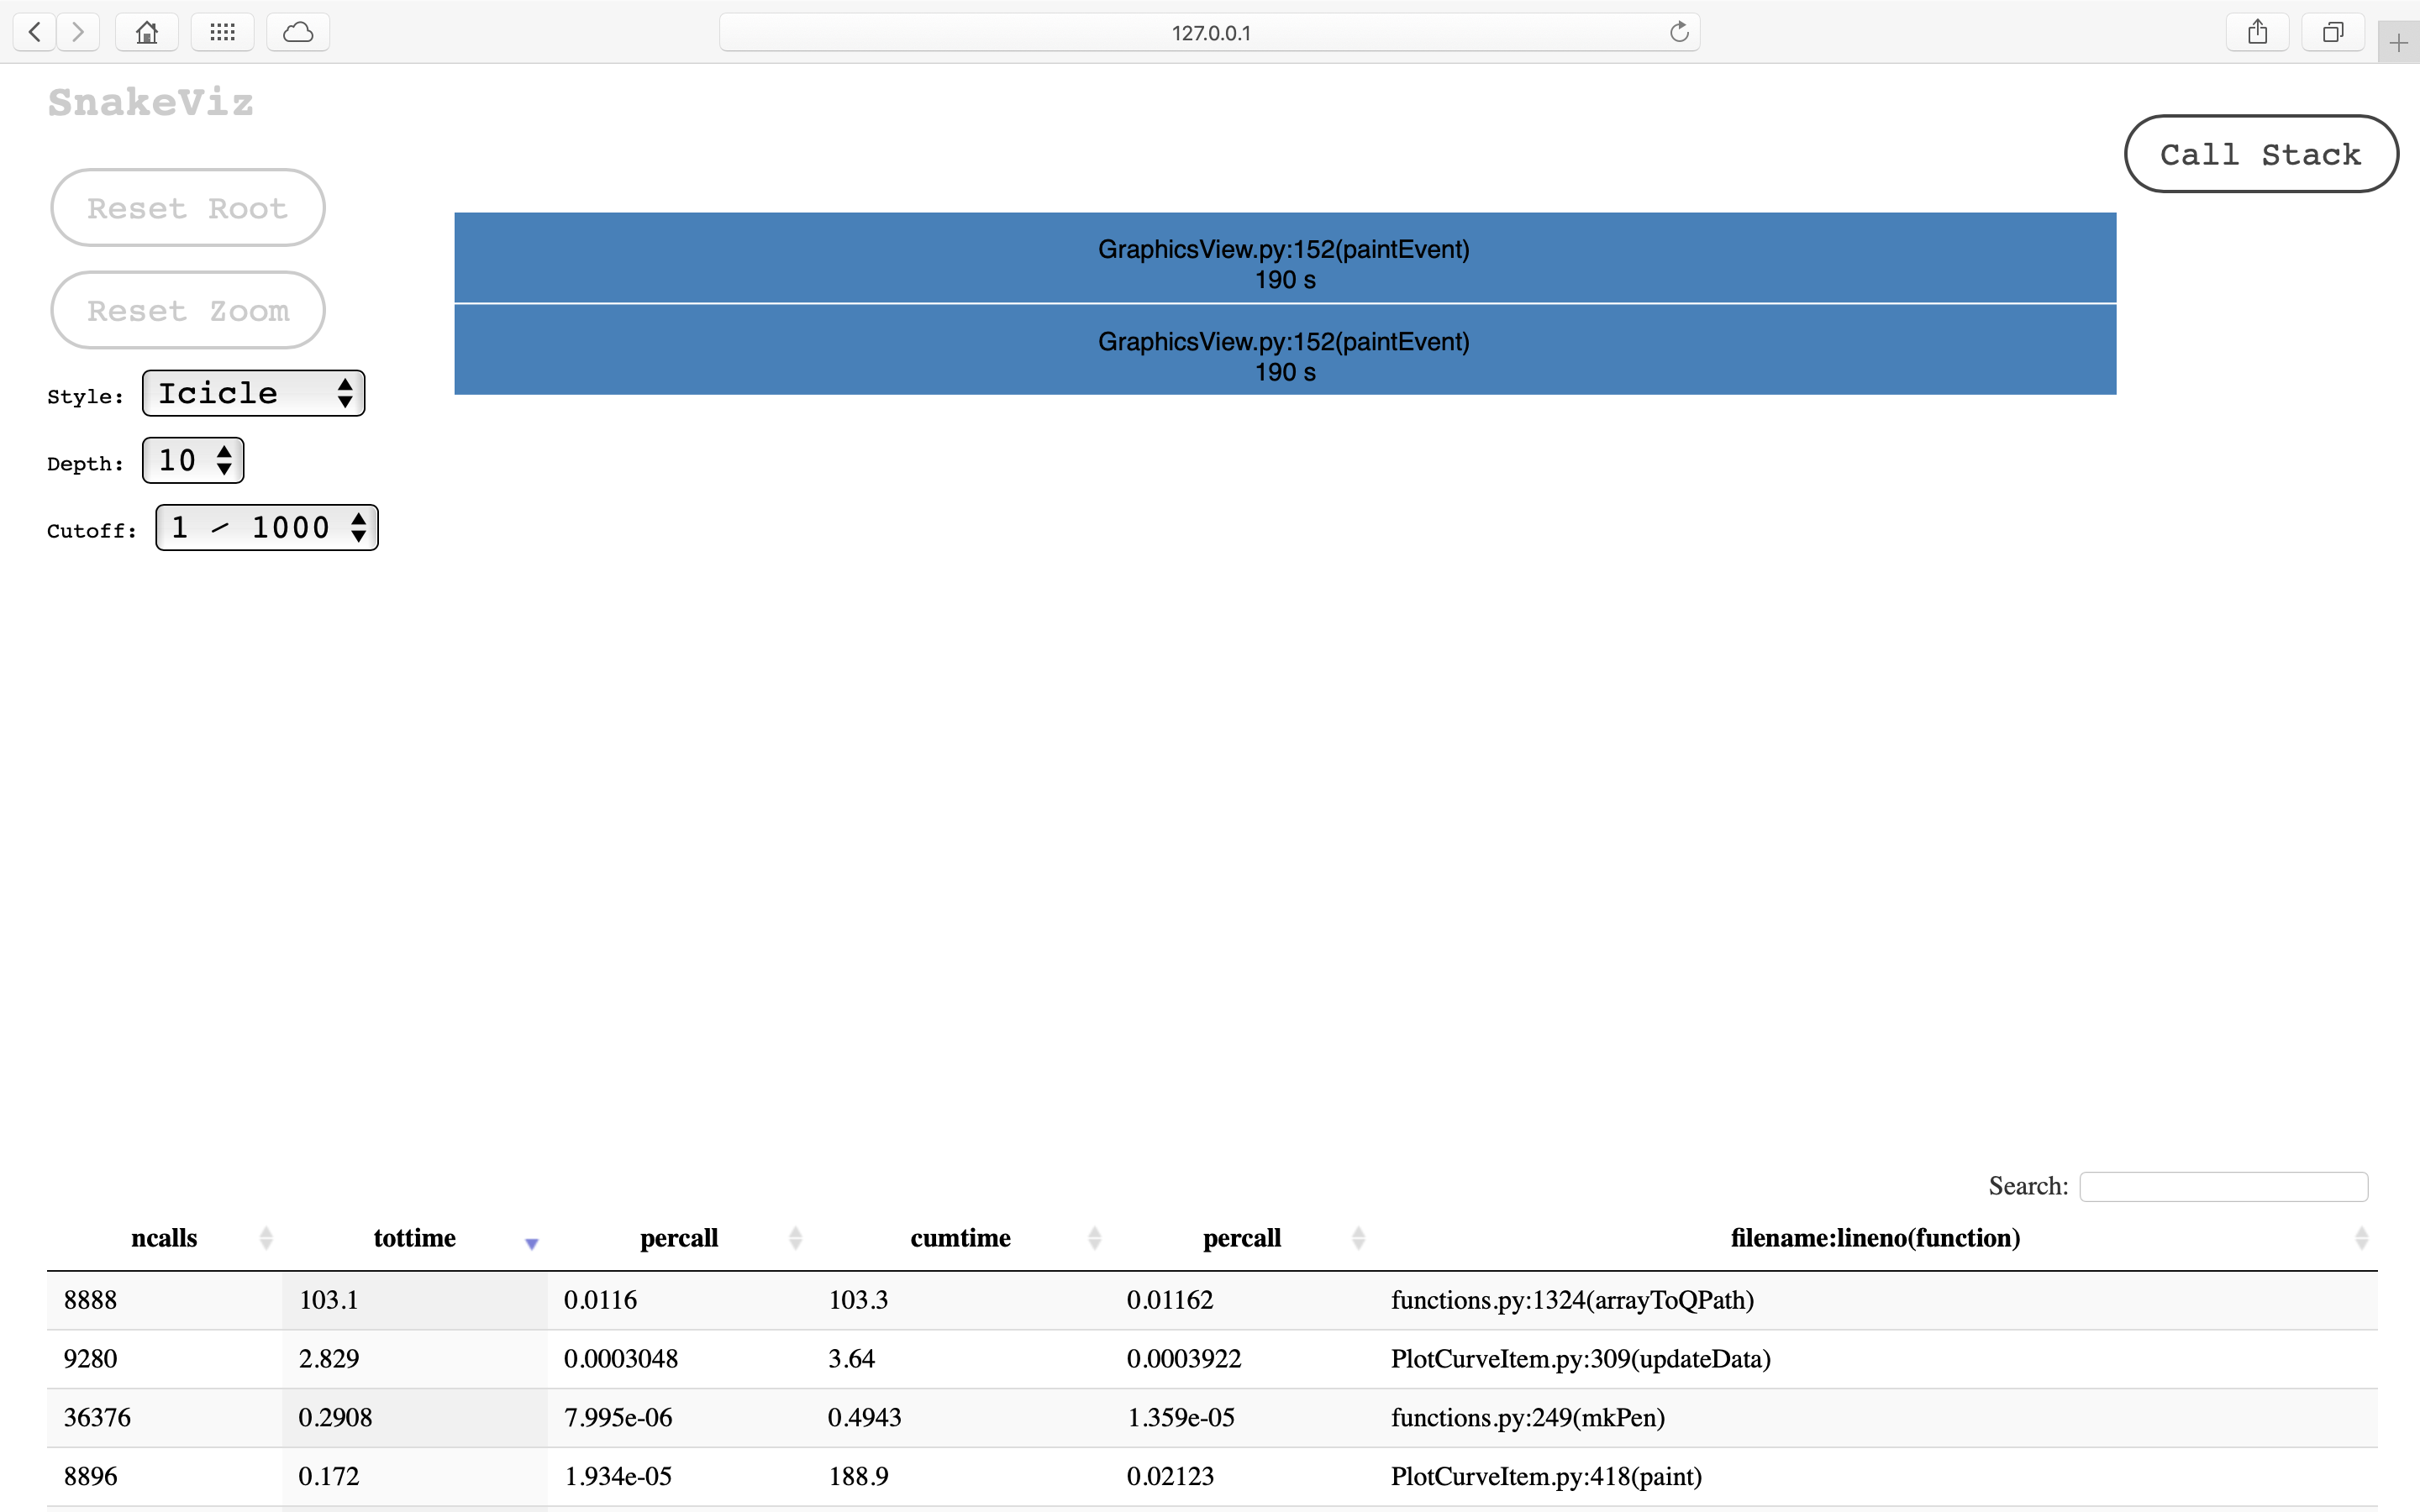
\includegraphics[width=15cm]{resources/img/profiles/HtProfile}
    \caption{Screenshot of the BE-CO-HT use case using Snakeviz}
    \label{fig:application:lhc:usecase:profile:ht}
\end{figure}

When it comes to scatter plots, another function does take quite some time as
well. A big amount of time is spent in the preparation of the symbol atlas,
which is a prerendered image of all symbols used in the scatter plot. When it
comes to rendering the actual plot, the already rendered symbols can simply be
copied from this atlas and pasted into the image. One potential way of improving
performance here is to bypass the loop over each data point in case all symbols
are the same. Screenshot \ref{fig:application:aps:usecase:profile:ht} shows the
profile of the \gls{aps} use case presented by Snakeviz in the browser.

\begin{figure}[h]
    \centering
    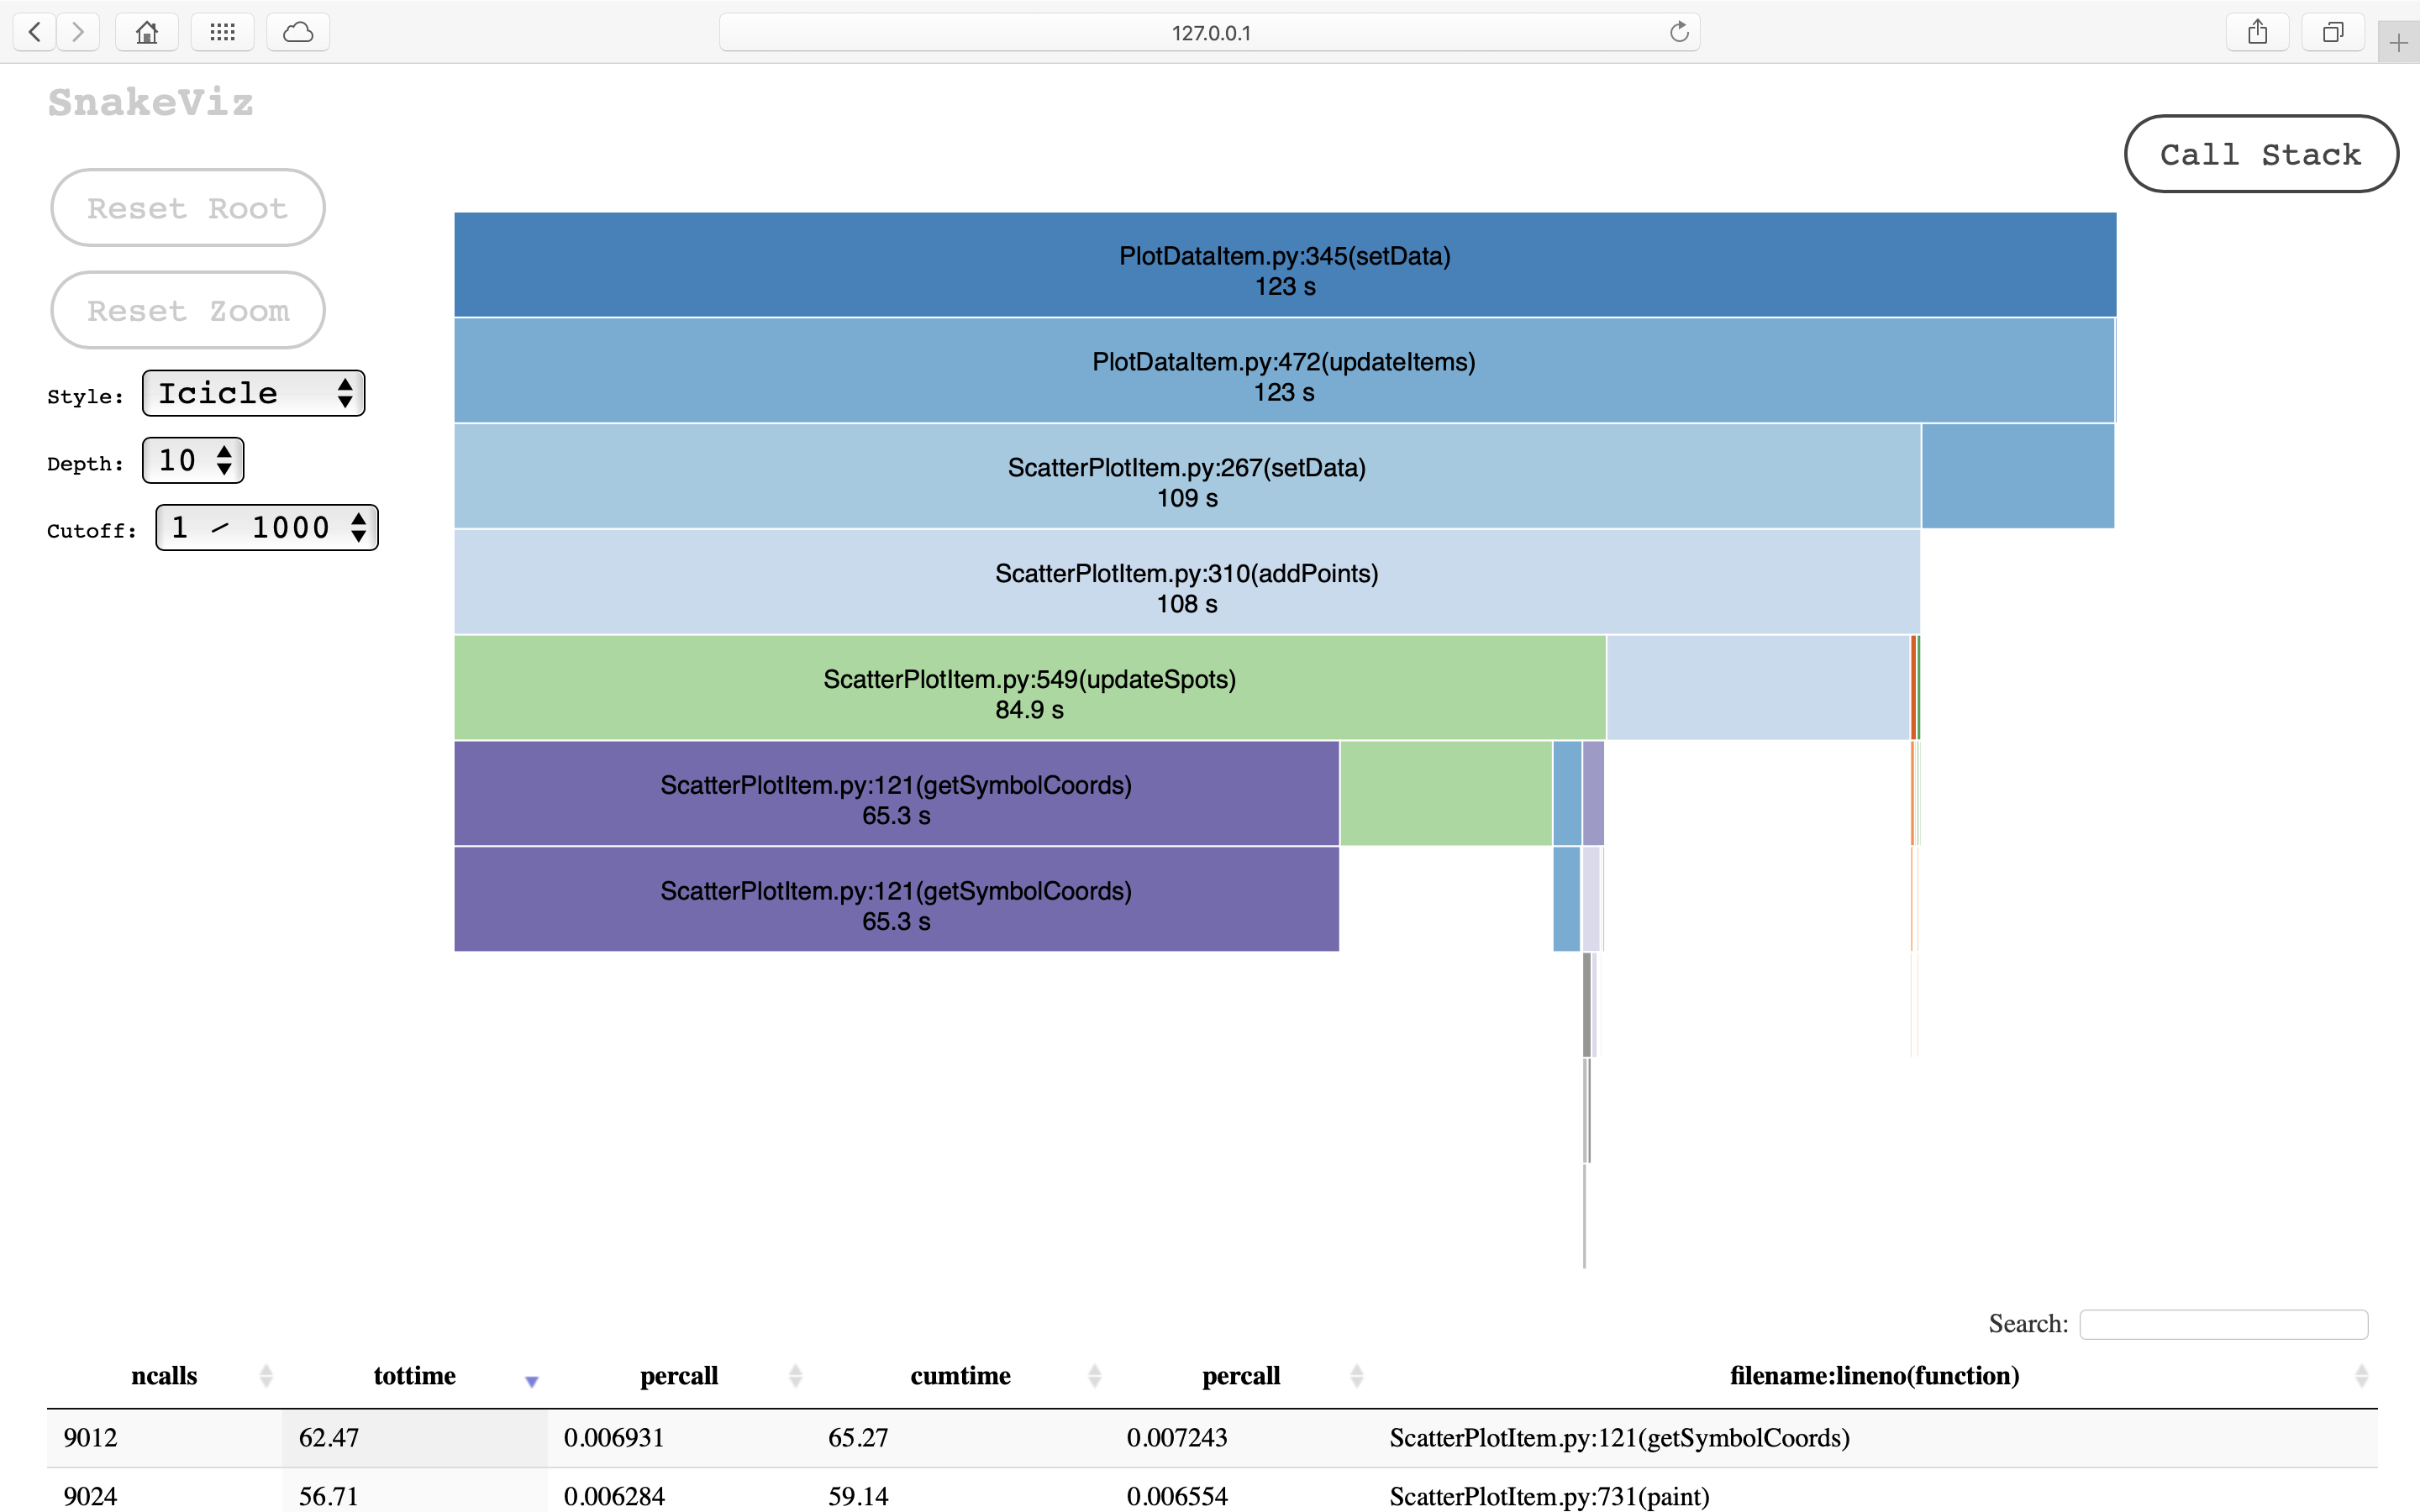
\includegraphics[width=15cm]{resources/img/profiles/ApsProfile}
    \caption{
        Screenshot of the BE-CO-APS use case's profile visualized in snakeviz
    }
    \label{fig:application:aps:usecase:profile:ht}
\end{figure}

\clearpage


%% ==============================================
%%          Performance Overhead
%% ==============================================


\section{Performance Overhead}

This chapter will focus on the evaluation of the framework. The biggest question
when it comes to evaluating performance of widgetmark is, how much overhead it
is adding compared to a standard application. The bigger our overhead is, the
more negative the results will be compared to the realistic value we can expect.

\subsection{Comparison Application}

To evaluate the accuracy of our benchmarking framework, we will compare the
times measured in a simple example use case with an actual implementation as a
minimal PyQt application. This application will only house a single plot updated
by the same conditions as the use case. To measure the timing in the
application, we will record a timestamp after each update. To find out how the
overhead of the framework develops under different load scenarios, we will use
different dataset size parameters for the plotting. For the evaluation we will
only choose a single plotting library, which will be PyQtGraph. The source code
for this application can be seen in listing \ref{listing:evaluation:pyqtapp}. It
is comprised of a single main window, containing the plot as its central widget.
The plot is a \inlinecode{Python}{pyqtgraph.PlotWidget()}, which is updated
using a \inlinecode{Python}{QtCore.QTimer} with a 0 second timeout, similar to
widgetmark's Qt executor class. Next to the data update, the current timestamp
is recorded on every timer timeout. As a hard coded barrier, 1000 redraws are
chosen. For every configuration, we have to executed the python module with
different parameters. The source code for the use case is appended in listing
\ref{listing:evaluation:usecase}. In both cases, the data generation are
excluded from time recording.

\subsection{Delta Time Accuracy}

Table \ref{tab:evaluation} compares the measured frame rates for each use case.
Both variants were executed on the same hardware with the same screen resolution
as well as the same window size. The measured data shows a trend of the
framework being slightly slower compared to the minimal PyQt application.

\begin{table}[h]
\begin{center}

\captionof{table}{
    Frame rate comparison between widgetmark and a minimal PyQt application
}
\label{tab:evaluation}

\begin{tabular}{rrrr}

\hline
Dataset Size & Widgetmark & PyQt Application & Overhead \\
\hline
1000         & 58.8       & 59.8             & 2.2\%    \\
10000        & 59.7       & 59.6             & 0\%      \\
500000       & 23.8       & 25.9             & 8.1\%    \\
1000000      & 12.5       & 13.9             & 10.1\%   \\
\hline

\end{tabular}
\end{center}
\end{table}

While these measurements already provide us with a general trend of the
framework adding a small overhead to our execution, it raises the question, how
this deviation compares with the fluctuation of the recorded times within a
execution. To compare this we first will have to get access to all measured
delta times for the PyQt application as well as the widgetmark run.

As a small rehearsal, we will quickly explain the sizes used in the following
detailed evaluation and why they are meaningful for us. The first important
measurement is the delta timing $\Delta t$, which describes the difference
between two measured adjacent time stamps. From a set of $m$ timestamps it can
be calculated for two adjacent timestamps $t_{i+1}$ and $t_i$ as:

$$\Delta t_{i} = t_{i+1} - t_{i}$$

The arithmetic mean or average $\bar{\Delta t}$ describes the average from our
set of $m-1$ measured delta times and is defined as:

$$\bar{\Delta t} = \frac{1}{m-1} * \sum_{i=0}^{m-1} {\Delta t_{i}}$$

The standard deviation $\sigma$ of our delta times describes, how far values are
deviated on average from $\bar{\Delta t}$. From the standard $\sigma$ we can get
a better idea if the measured times are very consistent or if they differ much
from each other. It is defined as:

$$ \sigma_{\Delta t} = \sqrt{\frac{1}{m-2} * \sum_{i=1}^{m-2} (\Delta t_{i} - \bar{\Delta t})^2} $$

The range of a set of $m-1$ delta times $\Delta t_i$ describes the difference
between the largest and smallest measured $\Delta t$ and is defined as:

$$R_{\Delta t} = \Delta t_{max} - \Delta t_{min}$$

Figures \ref{a:tab:evaluation:1000}, \ref{a:tab:evaluation:10000},
\ref{a:tab:evaluation:50000} and \ref{a:tab:evaluation:100000} compare all
measured delta times in the widgetmark as well as the minimal PyQt application.
For smaller dataset sizes, there are only small difference between both
noticeable. If the dataset size however increases, the difference measured in
the frame rates can be seen very well. In figure \ref{fig:evaluation:avg}, which
shows the average of the measured delta times, this difference becomes more
apparent.

\begin{figure}[h]
    \centering
    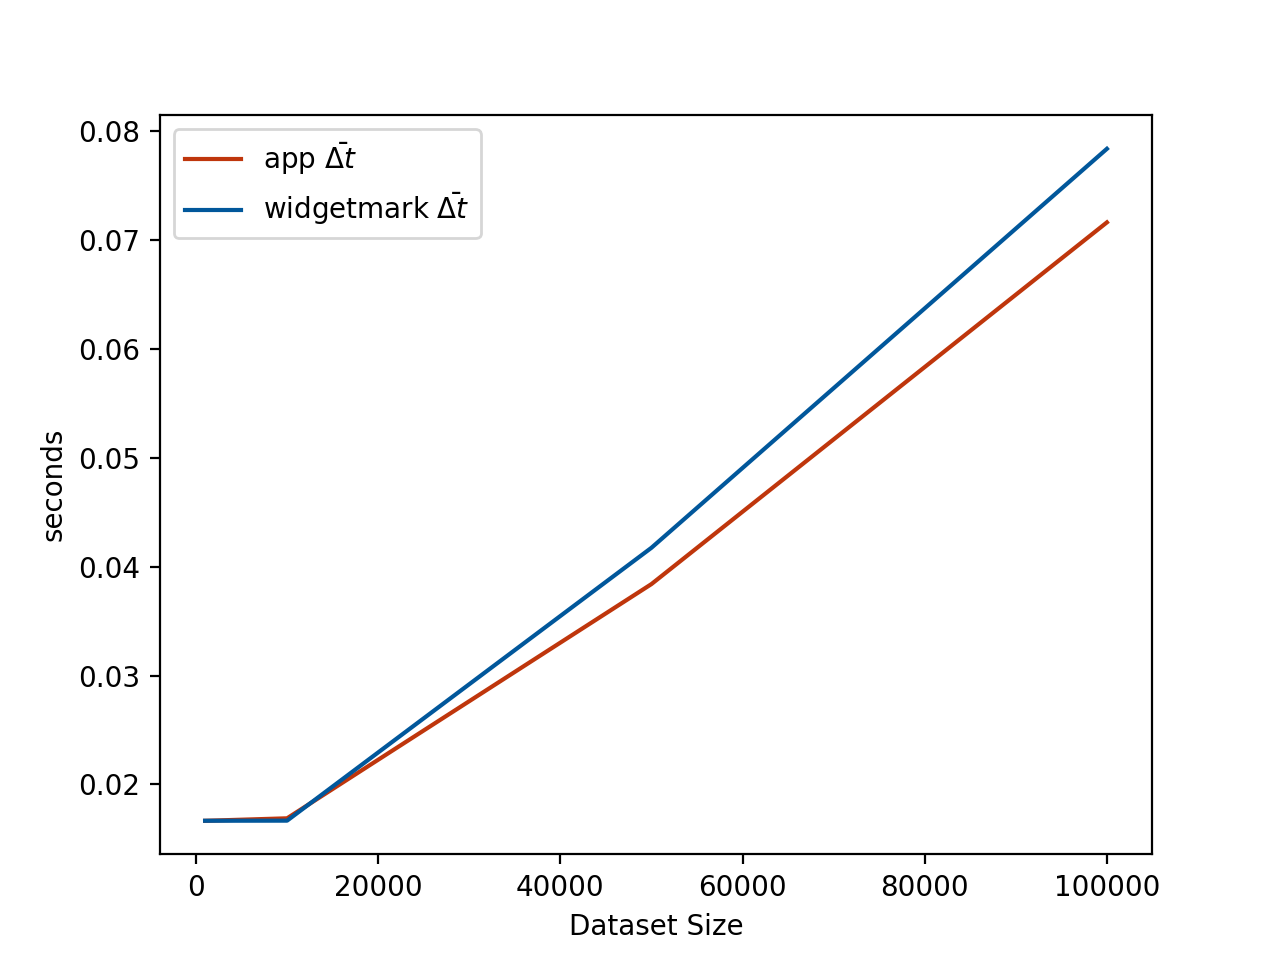
\includegraphics[width=12cm]{resources/img/evaluation/Eval_AVG}
    \caption{Average delta timing between both execution variants}
    \label{fig:evaluation:avg}
\end{figure}

Figure \ref{fig:evaluation:std} compares the difference between the average
delta times, the fluctuation of measured individual delta times and the ranges
$R_{\Delta t}$ of the framework as well as the minimal application. The
difference between widgetmark and the app in $\bar{\Delta t}$ is bigger compared
to their individual standard deviations $\sigma_{\Delta t}$. If it was in this
deviation range, it would be much more likely to be just a fluctuation in our
measurements. By clearly exceeding the expected deviation, we can assume that
the overhead will be reproducible, which supports our assumption, that
widgetmark does add an additional overhead to the execution, especially for
larger data set sizes. Compared to the measured value ranges $R_{\Delta t}$ of
each run, the difference is considerably smaller. These large ranges clearly
show, that it is very hard to further estimate, how high this actual overhead
will be on a run, since the recorded delta times can be very heavily influenced
by factors like the current load on the system. This is especially well
represented by the exceptional high range for the comparison application at
a data set size of $50000$ points. Additionally it shows the importance of a
reasonably high repeat counter, to keep the influence of such stray bullets as
small as possible.

\begin{figure}[h]
    \centering
    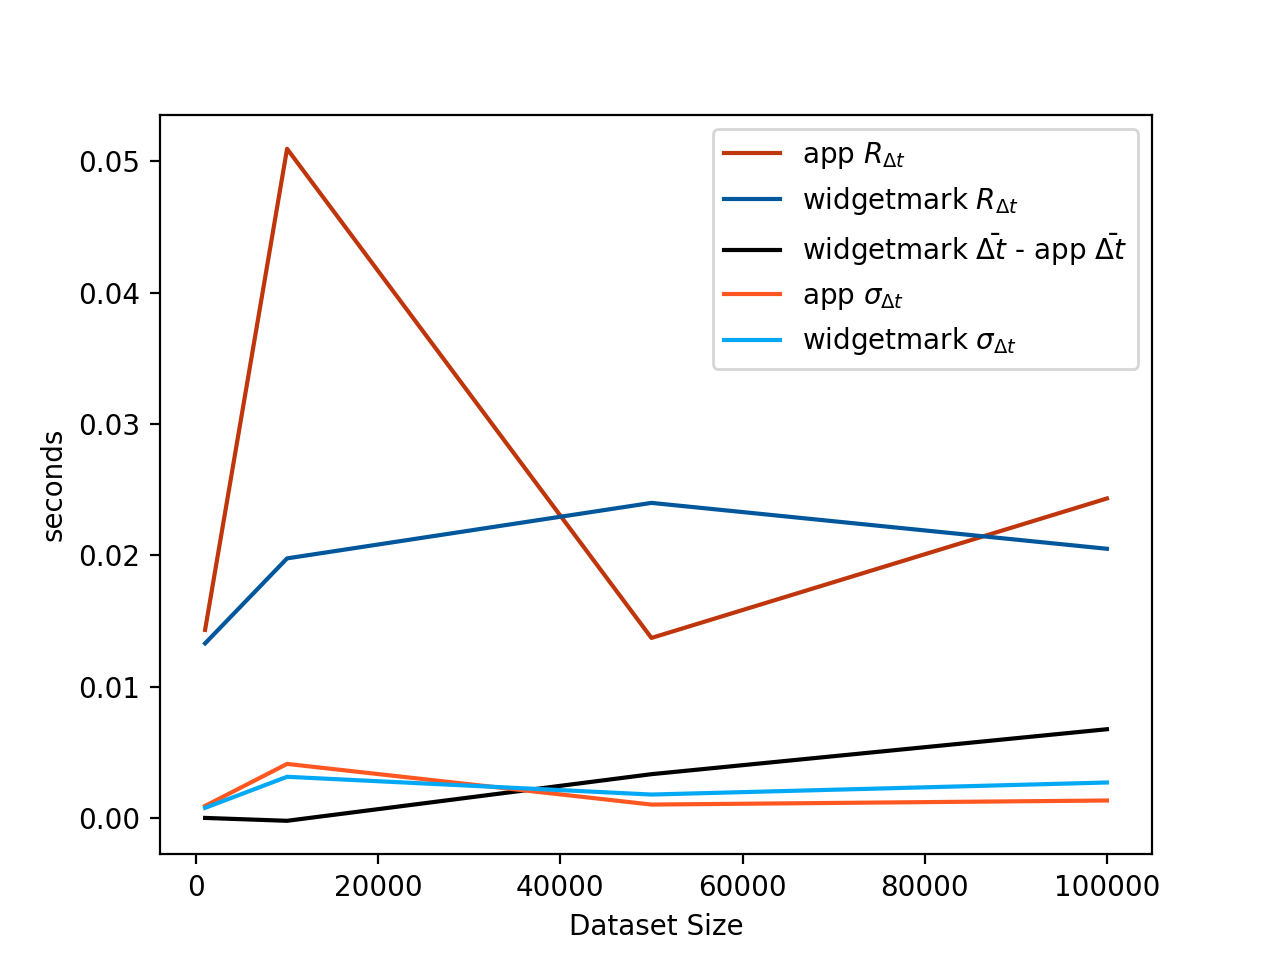
\includegraphics[width=12cm]{resources/img/evaluation/Eval_STD}
    \caption{Standard deviation compared to the delta timing value ranges and
        the average delta timing difference between both execution variants}
    \label{fig:evaluation:std}
\end{figure}

As a summary for the evaluation we can see, that widgetmark does add a slight
overhead to the executed use case. This overhead however does only slightly
influence the outcome of each use case, since it is still manages to represent
the libraries realistic performance capabilities.
